\documentclass[12pt,a4paper]{article}

% ─── Page Layout ───────────────────────────────────────────────────────────────
\usepackage[a4paper, margin=0.8in, headheight=14pt]{geometry}

% ─── Fonts (XeLaTeX) ───────────────────────────────────────────────────────────
\usepackage{fontspec}
\usepackage{unicode-math}
\setmainfont{TeX Gyre Pagella}
\setmonofont[Scale=0.88]{TeX Gyre Cursor}
\setmathfont{Latin Modern Math}

% ─── Packages ──────────────────────────────────────────────────────────────────
\usepackage{xcolor}
\usepackage{colortbl}
\usepackage{titlesec}
\usepackage{enumitem}
\usepackage{tabularx}
\usepackage{longtable}
\usepackage{booktabs}
\usepackage{array}
\usepackage{amsmath}
\usepackage{tikz}
\usetikzlibrary{shapes.geometric, arrows.meta, positioning, calc, fit, decorations.pathreplacing}
\usepackage{tcolorbox}
\tcbuselibrary{skins, breakable}
\usepackage{hyperref}
\usepackage{fancyhdr}
\usepackage{graphicx}
\usepackage{microtype}
\hyphenpenalty=10000
\exhyphenpenalty=10000
\sloppy
\usepackage{caption}
\usepackage{setspace}
\usepackage{multirow}
\usepackage{tocloft}

% ─── Q&A helper ────────────────────────────────────────────────────────────────
\newcommand{\Q}[1]{\textbf{#1}\par\noindent\ignorespaces}

% ─── Colour Palette ────────────────────────────────────────────────────────────
\definecolor{myred}{RGB}{196,30,58}
\definecolor{mydark}{RGB}{30,30,50}
\definecolor{mygreen}{RGB}{14,120,80}
\definecolor{myteal}{RGB}{0,130,140}
\definecolor{myamber}{RGB}{180,100,0}
\definecolor{mypurple}{RGB}{100,30,160}
\definecolor{mygray}{RGB}{246,247,249}
\definecolor{mgframe}{RGB}{180,185,200}
\definecolor{watermark}{RGB}{145,150,170}
\definecolor{hdrred}{RGB}{250,232,235}
\definecolor{hdrgreen}{RGB}{220,244,233}
\definecolor{hdrteal}{RGB}{220,242,244}
\definecolor{hdramber}{RGB}{253,242,215}
\definecolor{hdrpurple}{RGB}{238,228,255}
\definecolor{hdrgray}{RGB}{238,240,245}
\definecolor{rowalt}{RGB}{250,251,253}

% ─── Section Formatting ────────────────────────────────────────────────────────
\titleformat{\section}
  {\large\bfseries\color{myred}}{\thesection.}{0.5em}{}
  [\vspace{1pt}{\color{myred}\rule{\linewidth}{0.8pt}}]
\titleformat{\subsection}
  {\normalsize\bfseries\color{myteal}}{\thesubsection}{0.5em}{}
\titlespacing*{\section}{0pt}{18pt}{7pt}
\titlespacing*{\subsection}{0pt}{11pt}{4pt}

% ─── Paragraph ─────────────────────────────────────────────────────────────────
\setlength{\parindent}{0pt}
\setlength{\parskip}{4pt}

% ─── TOC Styling ───────────────────────────────────────────────────────────────
\renewcommand{\cfttoctitlefont}{\large\bfseries\color{myred}}
\renewcommand{\cftaftertoctitle}{\par\noindent{\color{myred}\rule{\linewidth}{0.8pt}}}
\setlength{\cftbeforetoctitleskip}{0pt}
\setlength{\cftaftertoctitleskip}{6pt}
\renewcommand{\cftsecfont}{\normalsize\bfseries\color{mydark}}
\renewcommand{\cftsecpagefont}{\normalsize\bfseries\color{mydark}}
\renewcommand{\cftsecleader}{\cftdotfill{\cftdotsep}}
\setlength{\cftbeforesecskip}{7pt}
\renewcommand{\cftsubsecfont}{\small\color{mydark}}
\renewcommand{\cftsubsecpagefont}{\small\color{mydark}}
\setlength{\cftbeforesubsecskip}{3pt}
\setlength{\cftsubsecindent}{1.4em}

% ─── Table helpers ─────────────────────────────────────────────────────────────
\renewcommand{\arraystretch}{1.45}
\setlength{\tabcolsep}{6pt}
\arrayrulecolor{mydark}
\newcolumntype{B}[1]{>{\small\bfseries\raggedright\arraybackslash}m{#1}}
\newcolumntype{Y}{>{\small\raggedright\arraybackslash}X}
\renewcommand{\tabularxcolumn}[1]{m{#1}}

% ─── Header / Footer ───────────────────────────────────────────────────────────
\pagestyle{fancy}
\fancyhf{}
\fancyhead[L]{\small\color{myred}\textbf{EC502}\;\color{mydark}--- Computer Architecture}
\fancyhead[R]{\small\color{myteal}\textbf{Module 6 Notes}}
\fancyfoot[C]{\small\color{mydark}\thepage}
\fancyfoot[R]{\small\color{watermark}\textit{\copyright\ Biraj}}
\renewcommand{\headrulewidth}{0.5pt}
\renewcommand{\footrulewidth}{0.3pt}

% ─── Hyperref ──────────────────────────────────────────────────────────────────
\hypersetup{
  colorlinks=true, linkcolor=myteal, urlcolor=myteal,
  pdfauthor={Biraj Sarkar},
  pdftitle={EC502 --- Module 6 Notes}
}

% ─── tcolorbox styles ──────────────────────────────────────────────────────────
\tcbset{
  tikzbox/.style={
    colback=mygray, colframe=mgframe, boxrule=0.6pt, arc=4pt,
    left=8pt, right=8pt, top=6pt, bottom=6pt,
    colbacktitle=mgframe, coltitle=mydark,
    fonttitle=\small\bfseries
  },
  defbox/.style={
    colback=hdrgreen, colframe=mygreen, boxrule=0.8pt, arc=4pt,
    left=9pt, right=9pt, top=6pt, bottom=6pt,
    colbacktitle=mygreen, coltitle=white,
    fonttitle=\small\bfseries
  },
  formulabox/.style={
    colback=hdrteal, colframe=myteal, boxrule=0.8pt, arc=4pt,
    left=9pt, right=9pt, top=7pt, bottom=7pt,
    colbacktitle=myteal, coltitle=white,
    fonttitle=\small\bfseries
  },
  examplebox/.style={
    colback=hdramber, colframe=myamber, boxrule=0.8pt, arc=4pt,
    left=9pt, right=9pt, top=6pt, bottom=6pt,
    colbacktitle=myamber, coltitle=white,
    fonttitle=\small\bfseries
  },
  masonbox/.style={
    colback=hdrpurple, colframe=mypurple, boxrule=0.8pt, arc=4pt,
    left=9pt, right=9pt, top=6pt, bottom=6pt,
    colbacktitle=mypurple, coltitle=white,
    fonttitle=\small\bfseries
  },
  exambox/.style={
    colback=hdrpurple, colframe=mypurple, boxrule=1pt, arc=5pt,
    left=10pt, right=10pt, top=8pt, bottom=8pt,
    colbacktitle=mypurple, coltitle=white,
    fonttitle=\bfseries,
    breakable, title after break={\textbf{Frequently Asked / Viva Questions (contd.)}}}
}
% Make all boxes breakable across pages
\tcbset{breakable}

% ─── TikZ styles ───────────────────────────────────────────────────────────────
\tikzset{
  block/.style={rectangle, draw=myteal, fill=hdrteal,
    text width=2.4cm, align=center, minimum height=0.95cm,
    font=\small, rounded corners=3pt, line width=0.7pt},
  redblock/.style={rectangle, draw=myred, fill=hdrred,
    text width=2.4cm, align=center, minimum height=0.95cm,
    font=\small, rounded corners=3pt, line width=0.7pt},
  netnode/.style={rectangle, draw=myteal, fill=hdrteal,
    text width=1.5cm, align=center, minimum height=0.8cm,
    font=\small, rounded corners=3pt, line width=0.7pt},
  sumjunc/.style={circle, draw=myamber, fill=hdramber,
    minimum size=0.62cm, font=\small, line width=0.8pt},
  snode/.style={circle, draw=mypurple, fill=hdrpurple,
    minimum size=0.55cm, font=\footnotesize, line width=0.7pt},
  arrow/.style={-Stealth, thick, color=mydark},
  redarrow/.style={-Stealth, thick, color=myred},
  line/.style={thick, color=mydark}
}

% ═══════════════════════════════════════════════════════════════════════════════
\begin{document}
% ═══════════════════════════════════════════════════════════════════════════════

\begin{center}
  {\LARGE\bfseries\color{myred} EC502 --- Computer Architecture}\\[5pt]
  {\normalsize\color{mydark} Semester V \quad$\bullet$\quad 3L:0T:0P \quad$\bullet$\quad 3 Credits}\\[3pt]
  {\normalsize\color{myteal}\textbf{Module 6 Exam Notes: System Organisation and Input Output}}\\[3pt]
  {\small\color{mydark} CGEC \;$|$\; B.Tech ECE (2023--27) \;$|$\; \textit{Biraj Sarkar}}
\end{center}
\vspace{2pt}
\noindent{\color{myred}\rule{\linewidth}{1.5pt}}
\vspace{2pt}

\hypersetup{linkcolor=mydark}
\tableofcontents
\hypersetup{linkcolor=myteal}
\newpage

\section{System Organisation and Input Output}
\begin{tcolorbox}[defbox,title={I/O interface and controller}]
An input/output (I/O) controller connects a device to the computer interconnect. It buffers data, reports status, accepts commands and adapts timing or protocol. A device driver tells the controller which operations the operating system wants.
\end{tcolorbox}
\subsection{Buses, controller registers and addressing}
\begin{itemize}[leftmargin=*,itemsep=3pt]
\item \textbf{Interconnection.} A shared bus carries address, data and control. A bus master initiates a transaction, while the selected target responds. A bridge joins buses or translates protocols and address ranges.
\item \textbf{Registers.} Data registers or FIFOs hold transfers. Status registers expose ready, busy, done or error. Control registers configure the device, start operations or enable interrupts. Read or write side effects depend on the device.
\item \textbf{Memory-mapped I/O.} An address range is decoded to device registers. Loads and stores access it. Device regions need the appropriate memory attributes and ordering rules because caching or reordering can change peripheral effects.
\item \textbf{Isolated or port-mapped I/O.} A separate I/O address space and special instructions or transaction types select a port. It can preserve memory address space, but requires separate ISA or bus support.
\end{itemize}
\par\vspace{6pt}\noindent
\begin{tabularx}{\linewidth}{|B{2.6cm}|Y|Y|}\hline
Feature & Memory-mapped I/O & Port-mapped I/O \\ \hline
Address allocation & Uses part of the memory address space. & Uses a separate port address space. \\ \hline
Instruction & Ordinary loads and stores with device access semantics. & Dedicated port operations or a distinct bus cycle. \\ \hline
Addressing modes & Can use the load/store modes allowed for device memory. & Limited to the modes offered by the port instructions. \\ \hline
\end{tabularx}

\begin{tcolorbox}[tikzbox,title={CPU, main memory and the peripheral interface},unbreakable]
\centering
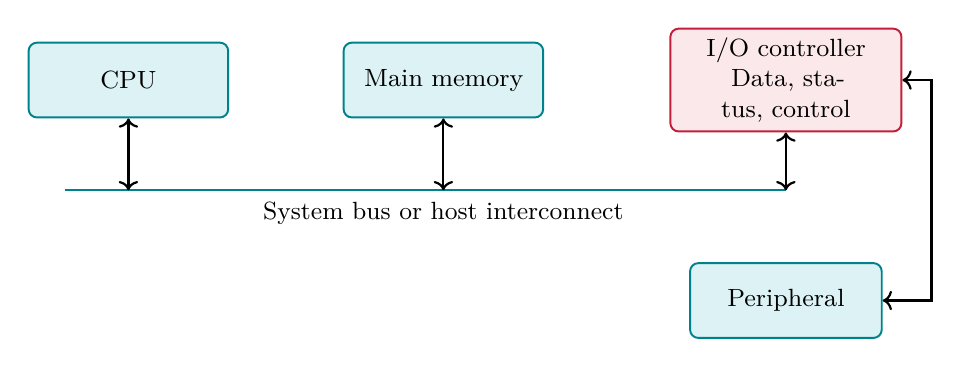
\begin{tikzpicture}[font=\small]
\node[block,text width=2.3cm] (cpu) at (0,0) {CPU};
\node[block,text width=2.3cm] (mem) at (4,0) {Main memory};
\node[redblock,text width=2.7cm] (ctl) at (8.35,0) {I/O controller\\Data, status, control};
\node[block,text width=2.2cm] (dev) at (8.35,-2.8) {Peripheral};
\draw[thick,myteal] (-.8,-1.4)--(8.35,-1.4);
\draw[<->,thick] (cpu.south)--(0,-1.4);
\draw[<->,thick] (mem.south)--(4,-1.4);
\draw[<->,thick] (ctl.south)--(8.35,-1.4);
\draw[<->,thick] (ctl.east)--(10.2,0)|-(dev.east);
\node[below] at (4,-1.42) {System bus or host interconnect};
\end{tikzpicture}
\end{tcolorbox}

\subsection{Synchronous and asynchronous transfer}
\begin{itemize}[leftmargin=*,itemsep=3pt]
\item \textbf{Synchronous bus.} Sender and receiver refer to agreed clock edges. An interface can add wait states until the target is ready. The shared protocol sets timing and direction for signals.
\item \textbf{Strobe.} A sender can assert data-valid without an acknowledgement if timing limits guarantee that the receiver can sample. This lacks explicit confirmation of completion.
\item \textbf{Handshaking.} A four-phase write starts when the source drives data and asserts request. The receiver latches stable data and asserts acknowledgement. The source deasserts request; the receiver then deasserts acknowledgement. This allows differing speeds. A practical clock-domain crossing needs appropriate synchronisation or an asynchronous FIFO.
\end{itemize}
\subsection{Arbitration}
When several masters request a shared bus, arbitration grants one at a time. In daisy-chain arbitration, a serial grant gives priority to the nearest requesting master. Parallel arbitration gives the arbiter separate requests and grants. Fixed priority can starve a low-priority master. Round robin rotates priority after service. Distributed arbitration lets contenders cooperate using a shared rule without one central grant controller.

\section{Programmed I/O and Interrupts}
\begin{tcolorbox}[defbox,title={Polling and interrupt}]
Polling asks the device repeatedly whether service is needed. An interrupt is a request that causes the CPU to suspend normal execution at an allowed point and transfer control to an interrupt service routine (ISR).
\end{tcolorbox}
\subsection{Programmed transfer and interrupt sequence}
\begin{enumerate}[leftmargin=*,itemsep=3pt]
\item \textbf{Programmed I/O.} The CPU issues a command, reads status until ready, and explicitly moves each item through a CPU register. Busy-waiting is simple but ties up the CPU.
\item \textbf{Interrupt request.} An enabled device raises a request. The interrupt controller may latch it and arbitrate priorities. The CPU accepts it at an architecture-defined point, usually an instruction boundary in a simple model.
\item \textbf{Enter ISR.} Save the return PC and required status. More registers may be saved by the ISR. In vectored I/O, a vector selects a handler or table entry. In a common-entry scheme, software polls pending status to identify the source.
\item \textbf{Complete service.} Read or write the controller, clear the cause and acknowledge completion where required. Restore state and execute interrupt return.
\end{enumerate}
\textbf{Priority and mask.} A mask controls which interrupts can be accepted. A non-maskable interrupt bypasses the ordinary mask for critical events. A priority controller may allow a higher-priority request to interrupt a lower-priority ISR. In a daisy-chained interrupt acknowledge, the first requesting device in the chain responds. A synchronous instruction exception is tied to the executing instruction, unlike an external device interrupt.

\begin{tcolorbox}[tikzbox,title={Daisy-chained interrupt acknowledgement},unbreakable]
\centering
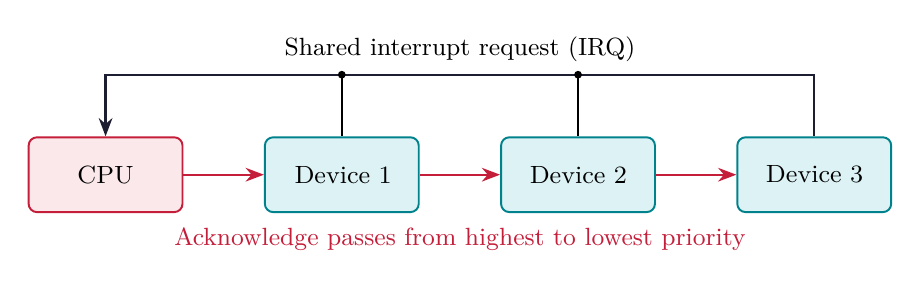
\begin{tikzpicture}[font=\small]
\node[redblock,text width=1.72cm] (cpu) at (0,0) {CPU};
\node[block,text width=1.72cm] (a) at (3.0,0) {Device 1};
\node[block,text width=1.72cm] (b) at (6.0,0) {Device 2};
\node[block,text width=1.72cm] (c) at (9.0,0) {Device 3};
\draw[redarrow] (cpu.east)--(a.west);
\draw[redarrow] (a.east)--(b.west);
\draw[redarrow] (b.east)--(c.west);
\draw[arrow] (c.north)--(9,1.27)--(0,1.27)--(cpu.north);
\draw[thick] (a.north)--(3,1.27) (b.north)--(6,1.27);
\fill (3,1.27) circle (1.4pt) (6,1.27) circle (1.4pt);
\node[above] at (4.5,1.31) {Shared interrupt request (IRQ)};
\node[below,myred] at (4.5,-.55) {Acknowledge passes from highest to lowest priority};
\end{tikzpicture}
\end{tcolorbox}

If Devices 2 and 3 request service together, Device 1 passes the acknowledgement along because it is idle. Device 2 claims it, supplies its vector and blocks the acknowledgement from Device 3. Device 3 can be serviced later. This fixes a physical priority order and can delay a device farther down the chain.

\begin{tcolorbox}[examplebox,title={Compare polling overhead with interrupt overhead}]
A 1 GHz CPU polls every $5\,\mu\mathrm s$ at 40 cycles per poll. Polling costs $200000(40)=8\times10^6$ cycles/s, or $0.8\%$ of CPU cycles. If the device instead interrupts at 4000 events/s with 300 cycles per service, cost is $1.2\times10^6$ cycles/s, or $0.12\%$. These estimates exclude common application processing. Polling response is bounded by the poll period in this simplified model. Interrupts have recognition and entry latency of their own.
\end{tcolorbox}

\section{Direct Memory Access}
\begin{tcolorbox}[defbox,title={Direct memory access}]
Direct memory access (DMA) transfers a block between a device and memory using a DMA-capable controller as bus master. The CPU sets up the transfer and handles completion, while the controller moves the data items.
\end{tcolorbox}
\begin{enumerate}[leftmargin=*,itemsep=3pt]
\item \textbf{Set up.} Driver supplies address or descriptors, length, direction and mode. A descriptor chain can describe multiple buffer segments.
\item \textbf{Request and grant.} Device or controller signals readiness. In a shared-bus model the DMA controller requests bus ownership and waits for a grant.
\item \textbf{Transfer.} DMA performs a device read plus memory write for input, or memory read plus device write for output, possibly as a direct combined transfer on suitable hardware. Update address and count after each unit.
\item \textbf{Finish.} Stop on terminal count or error, release bus ownership, and report status or interrupt the CPU. CPU and device must agree on when the buffer may be reused.
\end{enumerate}
\par\vspace{6pt}\noindent
\begin{tabularx}{\linewidth}{|B{3.05cm}|Y|Y|}\hline
Mode & Bus ownership & Typical trade-off \\ \hline
Burst & Controller holds bus for a block or bounded burst length. & Efficient block transfer, but CPU can wait longer for the bus. \\ \hline
Cycle stealing & Controller requests individual transfer cycles or small units. & Interleaves with CPU accesses while reducing available CPU bus cycles. \\ \hline
Transparent & Controller transfers only when the bus is otherwise idle. & Low CPU contention. Transfer completion time depends on idle availability. \\ \hline
\end{tabularx}

\begin{tcolorbox}[examplebox,title={DMA transfer time and contention}]
A $64\,\mathrm{KiB}$ block contains $16384$ 32-bit words. If the model completes one word per $20\,\mathrm{ns}$ bus cycle, data transfer takes $327.68\,\mu\mathrm s$. With $2\,\mu\mathrm s$ setup and no other stalls, total is $329.68\,\mu\mathrm s$. A single burst could occupy the bus for the data interval, while cycle stealing can spread bus use across time. It does not remove the number of data cycles needed.
\end{tcolorbox}

\textbf{Coherence and protection.} A DMA write changes memory and can leave a stale CPU cache copy. A DMA read can miss the latest dirty CPU data on a non-coherent system. Use platform-provided DMA synchronisation or hardware-coherent transfers. An I/O memory management unit (IOMMU) can translate permitted device addresses and constrain device access.

\section{Standard I/O Interfaces}
\begin{longtable}{|B{2.45cm}|>{\small\raggedright\arraybackslash}m{\dimexpr(\linewidth-2.45cm-6\tabcolsep-4\arrayrulewidth)/2\relax}|>{\small\raggedright\arraybackslash}m{\dimexpr(\linewidth-2.45cm-6\tabcolsep-4\arrayrulewidth)/2\relax}|}
\hline
Interface & Form and transaction model & Typical example \\ \hline
\endfirsthead
\hline
Interface & Form and transaction model & Typical example \\ \hline
\endhead
PCI & Conventional Peripheral Component Interconnect is a shared parallel expansion bus supporting configuration and bus mastering. & Legacy host expansion cards. \\ \hline
PCI Express & PCIe is a point-to-point serial packet interconnect. A root complex connects to endpoints directly or through switches. A link can contain multiple lanes. & Graphics cards, network adapters and NVMe storage. \\ \hline
USB & Universal Serial Bus is a host-controlled peripheral bus with hubs. The host enumerates devices, configures them and schedules transactions to endpoints. & Human interface devices, cameras and external storage. \\ \hline
SCSI / SATA & Small Computer System Interface (SCSI) defines a storage-oriented command model, historically used over parallel buses and now also carried over other transports. Serial ATA (SATA) is a point-to-point ATA storage link. & Disk and other storage connections. \\ \hline
RS-232 & Specifies electrical and interface signalling for serial equipment. A UART commonly supplies asynchronous start, data, optional parity and stop bits. A transceiver supplies the RS-232 electrical levels. & Serial terminals and instrumentation. \\ \hline
\end{longtable}

\textbf{USB transfer categories.} Control transfers configure devices and issue control requests. Bulk transfers move large reliable payloads without regular timing guarantees. Interrupt transfers get scheduled service opportunities for small periodic data, such as a keyboard. Isochronous transfers reserve periodic time for streams such as audio and do not retry missed packets at the transfer level. USB interrupt transfers are still scheduled by the host.

\newpage
\begin{center}
  {\large\bfseries\color{myred} Quick Revision --- Module 6}\\[3pt]
  {\small\color{mydark} System Organisation and Input Output $|$ EC502}
\end{center}
\noindent{\color{myred}\rule{\linewidth}{1.2pt}}
\begin{tcolorbox}[formulabox,title={Key Formulas at a Glance}]
\renewcommand{\arraystretch}{1.35}
\begin{tabularx}{\linewidth}{B{5.0cm}Y}
Polling demand & Poll frequency times cycles per poll \\[3pt]
Interrupt demand & Interrupts per second times cycles per service \\[3pt]
DMA data time & Transfer units times time per unit in a no-stall model \\[3pt]
Shared bus & Only the granted master initiates the shared transaction \\[3pt]
\end{tabularx}
\end{tcolorbox}
\begin{tcolorbox}[defbox,title={One-Line Definitions}]
\textbf{Interrupt vector.} Number or address used to select the corresponding handler.\par
\textbf{DMA.} Controller-driven data movement between memory and a device without a CPU copy per item.\par
\textbf{Handshaking.} Exchange of request and acknowledgement signals to coordinate a transfer.\par
\end{tcolorbox}
\begin{tcolorbox}[exambox,title={Frequently Asked / Viva Questions}]
\begin{enumerate}[topsep=0pt, label=\textbf{Q\arabic*.}, itemsep=5pt]
\item \Q{What is the difference between device status and control registers?}
Status reports controller state. Control registers configure or command it.
\item \Q{How does memory-mapped I/O select a device?}
Address decoding directs loads or stores to the device register range.
\item \Q{Why can synchronous buses still need wait states?}
A target may require extra cycles before data is ready.
\item \Q{What limits fixed-priority arbitration?}
Frequent high-priority requests can starve lower-priority masters.
\item \Q{How is a vector useful?}
It directs service to the appropriate ISR without searching every device.
\item \Q{Why does an ISR save state?}
Normal execution must resume with the required architectural state restored.
\item \Q{Does interrupt-driven I/O automatically imply DMA?}
No. An ISR can still move each item through a CPU register.
\item \Q{What is cycle stealing?}
DMA temporarily obtains a bus cycle or small group of cycles between other masters' accesses.
\item \Q{How do PCI and PCIe differ?}
Conventional PCI is a shared parallel bus. PCIe uses serial point-to-point links.
\item \Q{Which USB mode suits a real-time audio stream?}
Isochronous transfer, which provides periodic service opportunities.
\end{enumerate}
\end{tcolorbox}
\begin{tcolorbox}[tikzbox,title={Summary comparison}]
\begin{tabularx}{\linewidth}{|B{4cm}|Y|}\hline
\textbf{Case} & \textbf{What to use} \\ \hline
Polling & CPU waits or checks periodically, then moves data. \\ \hline
Interrupt-driven & Device requests CPU service when ready. CPU may still copy items. \\ \hline
DMA & CPU sets up a block transfer, and the controller moves the data. \\ \hline
\end{tabularx}
\end{tcolorbox}
\end{document}
